\documentclass{standalone}
\usepackage{tikz}
\begin{document}

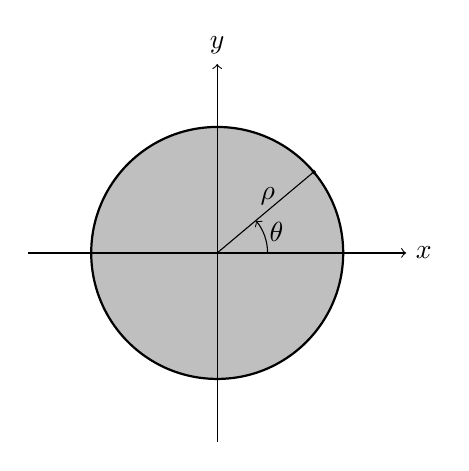
\begin{tikzpicture}[scale=2]

  \def\r{0.8}      % radius
  % Circle
  \filldraw[fill=lightgray, thick] (0,0) circle (\r);

  % Draw axes
  \draw[->] (-1.2,0) -- (1.2,0) node[right] {$x$};
  \draw[->] (0,-1.2) -- (0,1.2) node[above] {$y$};

  % Polar coordinates
  \def\thetaval{40} % angle in degrees

  % Point in polar coordinates
  \coordinate (P) at (\thetaval:\r);

  % Draw angle arc
  \draw[->] (0.4*\r,0) arc[start angle=0, end angle=\thetaval, radius=0.4*\r];
  \node at (\thetaval/2: 0.5*\r) {$\theta$};
  \draw (0,0) -- (P) node[pos=0.7, anchor=east] {$\rho$};
  
  % Mark the point
  \filldraw[] (P) circle (0.01);

\end{tikzpicture}

\end{document}
